\documentclass[border=4pt]{standalone}
\usepackage{pgfplots}
\pgfplotsset{compat=1.17}
\begin{document}
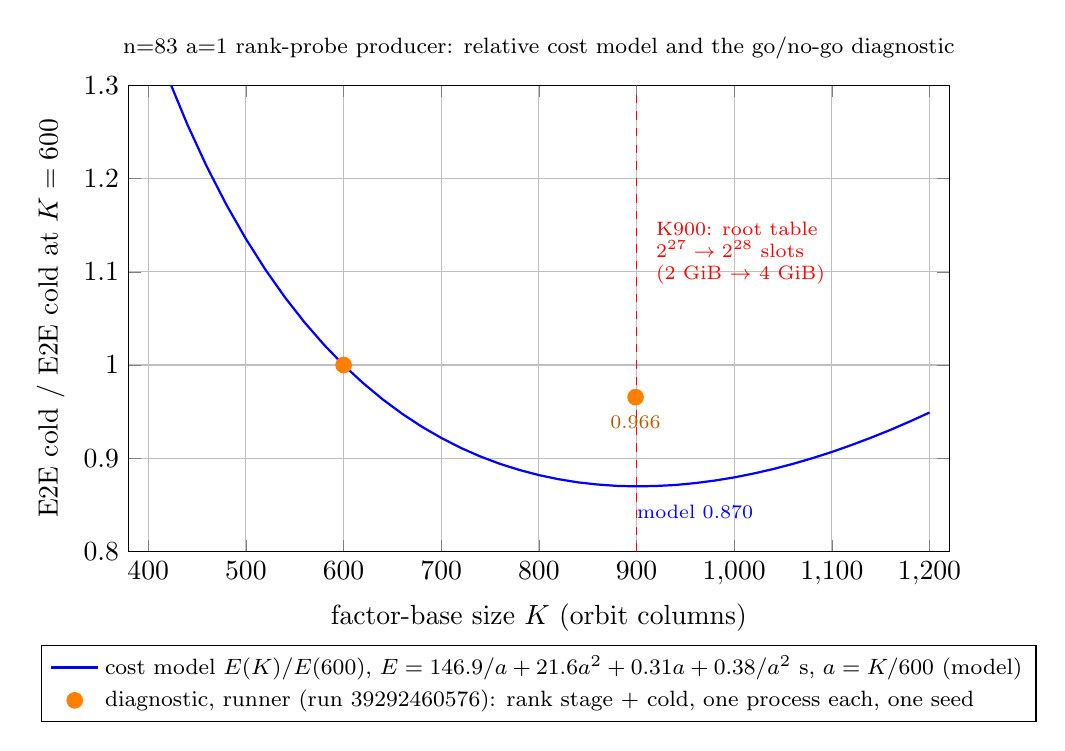
\begin{tikzpicture}
\begin{axis}[width=12cm,height=7.5cm,xlabel={factor-base size $K$ (orbit columns)},
 ylabel={E2E cold / E2E cold at $K=600$},xmin=380,xmax=1220,ymin=0.8,ymax=1.3,grid=major,
 legend style={font=\footnotesize,at={(0.5,-0.2)},anchor=north,cells={anchor=west}},
 title={\footnotesize n=83 a=1 rank-probe producer: relative cost model and the go/no-go diagnostic}]
\addplot[blue,thick] coordinates {(400,1.3654) (420,1.3088) (440,1.2582) (460,1.2128) (480,1.1720) (500,1.1353) (520,1.1023) (540,1.0726) (560,1.0458) (580,1.0217) (600,1.0000) (620,0.9806) (640,0.9632) (660,0.9477) (680,0.9339) (700,0.9218) (720,0.9111) (740,0.9019) (760,0.8940) (780,0.8874) (800,0.8819) (820,0.8775) (840,0.8741) (860,0.8718) (880,0.8703) (900,0.8698) (920,0.8702) (940,0.8713) (960,0.8733) (980,0.8760) (1000,0.8794) (1020,0.8836) (1040,0.8884) (1060,0.8939) (1080,0.9000) (1100,0.9067) (1120,0.9141) (1140,0.9220) (1160,0.9304) (1180,0.9395) (1200,0.9490)};
\addlegendentry{cost model $E(K)/E(600)$, $E = 146.9/a + 21.6a^2 + 0.31a + 0.38/a^2$ s, $a=K/600$ (model)}
\addplot[only marks,mark=*,mark size=2.8pt,orange] coordinates {(600,1) (899,0.9655)};
\addlegendentry{diagnostic, runner (run 39292460576): rank stage + cold, one process each, one seed}
\draw[dashed,red] (axis cs:899.5,0.8) -- (axis cs:899.5,1.3);
\node[red,font=\scriptsize,anchor=west,align=left] at (axis cs:910,1.12) {K900: root table\\$2^{27}\to2^{28}$ slots\\(2 GiB $\to$ 4 GiB)};
\node[orange!70!black,font=\scriptsize,anchor=north] at (axis cs:899,0.9555) {0.966};
\node[blue,font=\scriptsize,anchor=north] at (axis cs:960,0.8598) {model 0.870};
\end{axis}
\end{tikzpicture}
\end{document}
